\documentclass[12pt,a4paper]{article}
\usepackage[utf8]{inputenc}
\usepackage{amsmath}
\usepackage{amsfonts}
\usepackage{amssymb}
\usepackage{graphicx} 
\usepackage{subcaption}
\usepackage[margin=2cm]{geometry}

\newtheorem{theorem}{\bf Theorem}
\newtheorem{todo}{\bf Todo}
\newtheorem{remark}{\bf Remark}
\newtheorem{corollary}{\bf Corollary}
\newtheorem{definition}{\bf Definition}
\newtheorem{lemma}{\bf Lemma}
\newtheorem{proposition}[theorem]{\bf Proposition}

\begin{document}


\begin{figure}[tp]	
\centering
	\begin{subfigure}{0.7\textwidth}
		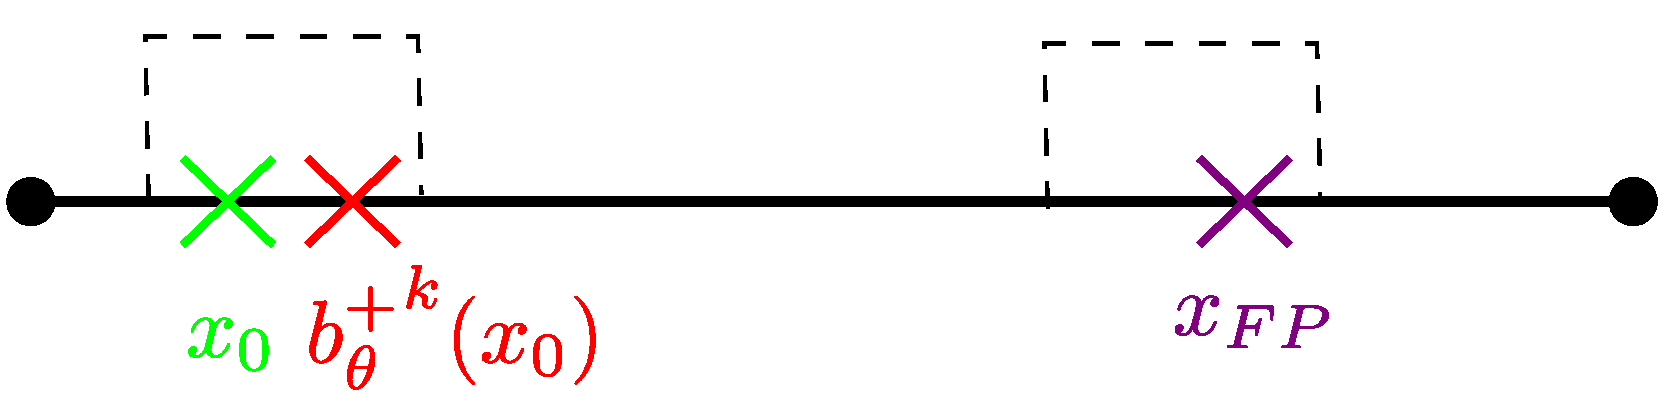
\includegraphics[width=1.0\textwidth]{a.pdf}
		\caption{Slow convergence: finds a cycle that is not a periodic orbit.}
		\label{fig:a}
	\end{subfigure}\\
	\begin{subfigure}{.7\textwidth}
		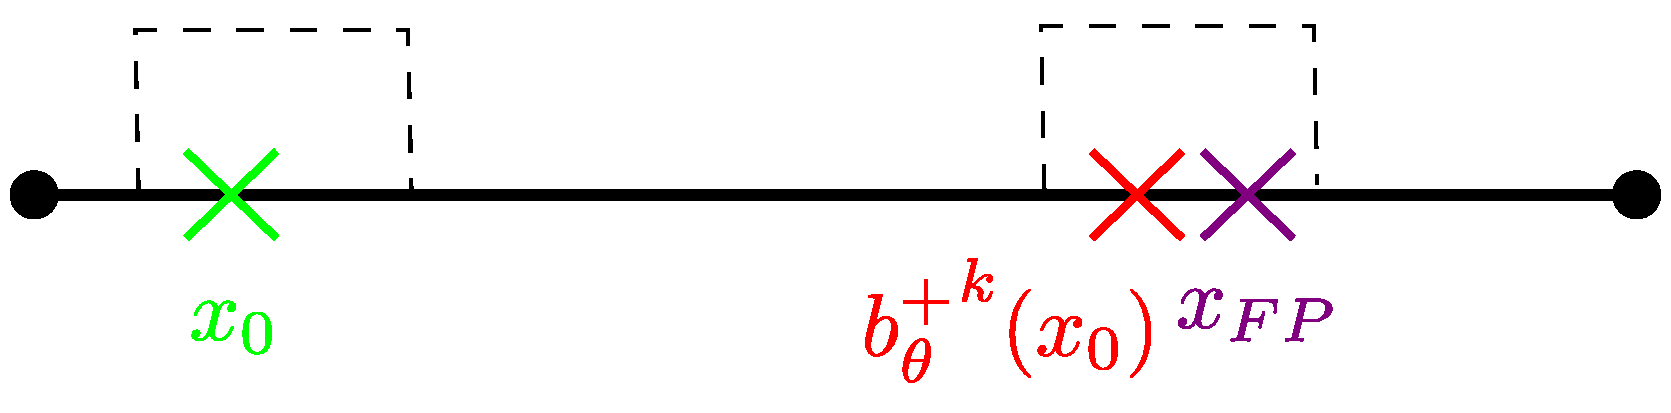
\includegraphics[width=1.0\linewidth]{b.pdf}
		\caption{Fast convergence: finds the real periodic orbit.}
		\label{fig:b}
	\end{subfigure}\\
	\begin{subfigure}{.7\textwidth}
		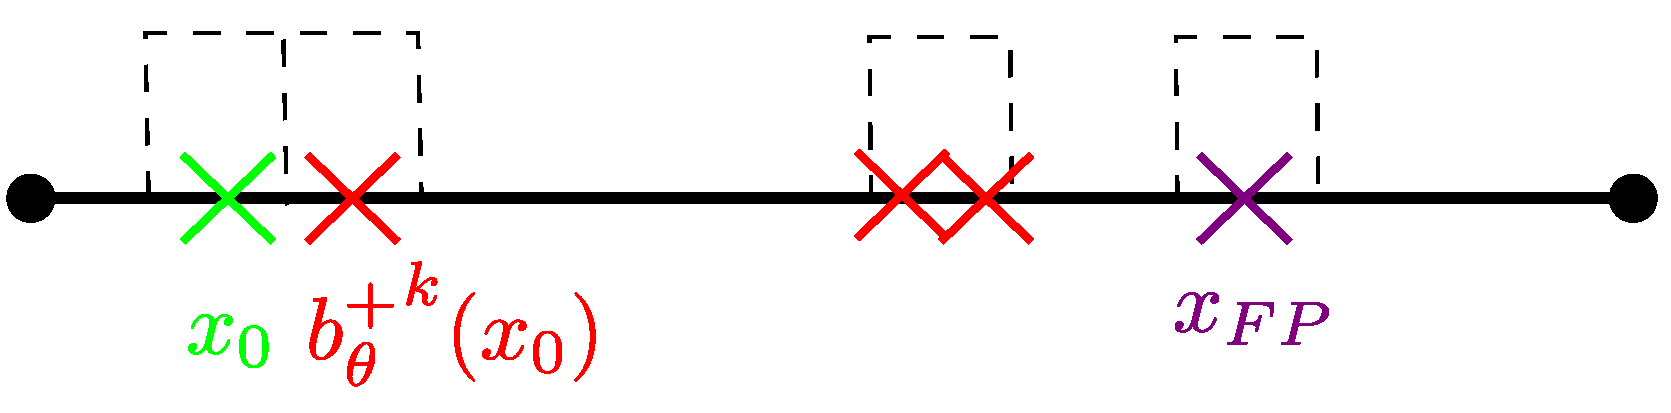
\includegraphics[width=1.0\linewidth]{c.pdf}
		\caption{Increasing resolution can still lead to false cycle detection as we
approach the fixed point.}
		\label{fig:c}
	\end{subfigure}\\
	\begin{subfigure}{.7\textwidth}
		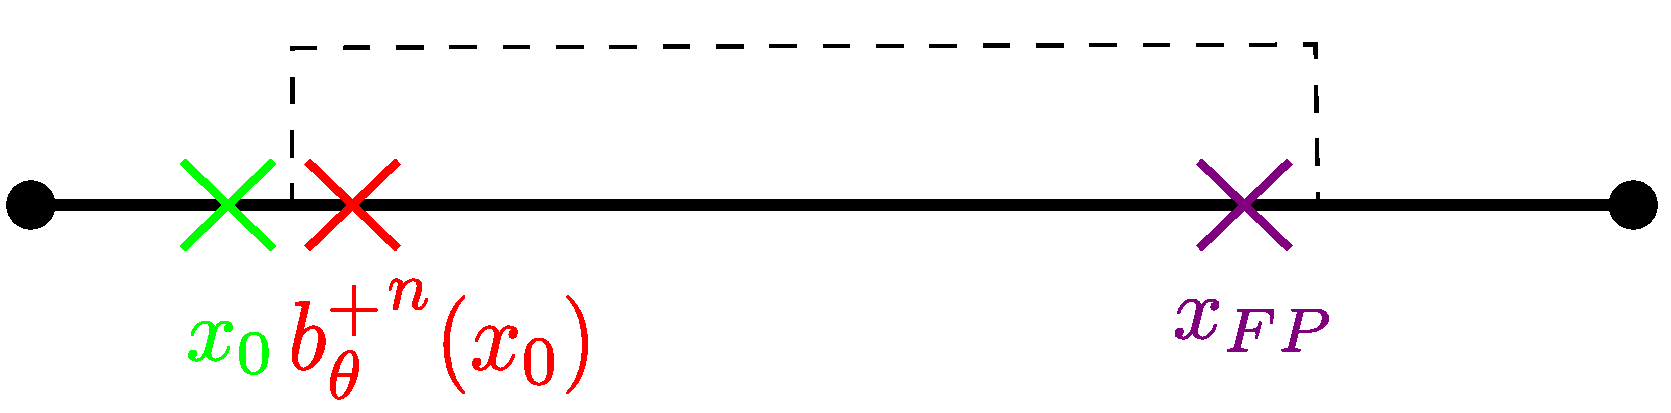
\includegraphics[width=1.0\linewidth]{d.pdf}
		\caption{Decreasing resolution can lead to finding correct cycle, with lower
spatial resolution.}
		\label{fig:d}
	\end{subfigure}%
	\caption{Resolution analysis.}
	\label{fig:resolution}	
\end{figure}

We explore the trade-off between spatial resolution and correctness of cycle
detection with a discretized approach to fixed-angle bouncing.

In Figure \ref{fig:resolution} we show an edge length $l$ for a given $n$-gon
(polygon with $n$ sides). We assume that the robot hits that edge for the first
time at point $x_0$ and that there exists a stable limit cycle of period $n$
that hits the edge at point $x_{FP}$. Let ${b^+_{\theta}}^{k}(x_0)$ be the hit
point on the polygon boundary after iterating $k$ times the bouncing map
${b^+_{\theta}}(x_0)$, starting from $x_0$. Finally, we show as dotted squares
the cells for a given discretization.

In regular polygons, for certain intervals of $\theta$, only one stable limit cycle
exists. When the discretized limit-cycle finding algorithm finds more than one periodic orbit, only one
of them can be the true limit cycle. The other orbits appear as an artefact of
the current discretization resolution. For certain values of $\theta$, the
convergence rate towards $x_{FP}$ is quite small, resulting in successive collision points
${b^+_{\theta}}^{k}(x_0)$ that slowly move away from $x_0$. For example,
consider Figure \ref{fig:a} and assume that ${b^+_{\theta}}^{k}(x_0)$ has
already returned to the edge containing the start point $x_0$. For a given resolution and a certain
$\theta$, $x_0$ and ${b^+_{\theta}}^{k}(x_0)$ can fall in the same cell $z$,
which would result into an apparent periodic orbit, but $z$ is indeed a
transient cell. Conversely, in Figure \ref{fig:b}, the algorithm has iterated
enough (or convergence is fast enough) such that ${b^+_{\theta}}^{k}(x_0)$ and $x_{FP}$ are in the same cell
$z$, so $z$ is truly a persistent cell (all future bounces on this edge will be
in $z$).

To avoid the issue present in Figure \ref{fig:a}, the discretization resolution
could be increased such that $x_0$ and ${b^+_{\theta}}^{k}(x_0)$ fall into
different cells $z$ and $w$, just as seen in Figure \ref{fig:c}, therefore, $z$
and $w$ would be classified as transient cells. Nonetheless, with this finer
discretization it is still possible that as ${b^+_{\theta}}^{k}(x_0)$ keeps
iterating, two consecutive collision points ${b^+_{\theta}}^{jn}(x_0)$ and
${b^+_{\theta}}^{(j+1)n}(x_0)$ will fall in
the same cell, and we still detect a spurious periodic cycle. The resolution could
again be increased but this also has the inconvenience that as the cells become
smaller, the algorithm will need more iterations in order to find the real
stable limit cycle. And there is no clear way to choose a discretization fine
enough to guarantee no false cycles..

Based on the last analysis it is desirable to have large enough cells to avoid
over iterating the algorithm, but we want to have the smallest cells possible
(to have good spatial resolution of the location of the limit cycle in the
workspace).

Inequality (\ref{eq:dist_bound}) can be used to compute an actual bound for the
distance between ${b^+_{\theta}}^{k}(x_0)$ and $x_{FP}$ as a function of $k$.
We set $k=n$, as the minimum $k$ that returns the robot to the
edge where $x_0$ is located, opening the possibility of closing a cycle. Thus,
the quantity $c(\theta)^n l$ is an upper bound for the distance between
${b^+_{\theta}}^n(x_0)$ (the first collision point where the robot returns to the
 edge it started on) and $x_{FP}$. If chosen as the discretization length, we
are guaranteed to detect only one cycle (the correct one).

For an example, suppose that in Figure \ref{fig:b}, the point
${b^+_{\theta}}^{k}(x_0)$ has $k=n$. If that is the case, it can be seen that
the shown cell size is enough to contain distance
$d({b^+_{\theta}}^{n}(x_0),x_{FP})$, so the algorithm would not identify
spurious periodic orbits and would rapidly find the persistent cell that
contains $x_{FP}$. On the other hand, if the distance between
${b^+_{\theta}}^{n}(x_0)$ and $x_{FP}$ is larger, it would require bigger cells
just as shown in Figure \ref{fig:d}. In either case, selecting the cell size
according to distance $d({b^+_{\theta}}^{n}(x_0),x_{FP})$ (actually according to
its bound $c(\theta)^{n} l$), makes the algorithm identify a single limit cycle
with fewer iterations.

If we want better spatial resolution, we can ignore any limit cycles detected
in the first $jn$ collisions, and choose a discretization of $c(\theta)^{jn}
d(x_0, x_{FP})$. This lets us tune the spatial resolution to be finer without
detecting false cycles.

\textbf{Caveats:} This is only for regular polygons, and assumes that the
discretization is rectilinear to the polygon boundary (which may only be true
for one side). Uneven overlaps between the polygon boundary and the
discretization may still cause false cycles to be found.

\begin{theorem} \label{Proposition:distanceFromFP}
Assume an adjacent edges fixed bouncing scheme, and assume that the robot starts
over $\delta P$ at distance $x_0 \in (0,l)$ from vertex $v_i$. When the robot
encounters $\delta P$ for the $k^{\text{th}}$ time, then \begin{equation}
\label{eq:dist_bound}
d({b^+_{\theta}}^{k}(x_0),x_{FP}) < c(\theta)^{k} l.
\end{equation}
\end{theorem}
\begin{corollary} \label{rm1}
If the initial distance $x_0$ is known, then $c(\theta)^{k} d(x_0,x_{FP})$ gives
the exact bound to $d({b^+_{\theta}}^{k}(x_0),x_{FP})$ . 
\end{corollary}


\end{document}
